\documentclass[14pt, singlecolumn, citestyle=authoryear]{elegantbook}
\definecolor{pink}{RGB}{125, 33, 217}
\definecolor{href}{RGB}{255, 0, 120}
\definecolor{customcolor}{RGB}{252, 3, 252}
\colorlet{coverlinecolor}{customcolor}
\usepackage[english, russian]{babel}
\usepackage{graphicx}
\usepackage{svg}
\usepackage{booktabs}
\begin{document}
\mainmatter


\makeatletter
\patchcmd{\chapter}{\if@openright\cleardoublepage\else\clearpage\fi}{}{}{}
\makeatother



\chapter*{\textbf{\huge \textcolor{black}{Исследование распределения степени линейной поляризации на небе. Поляризационный компас}}}

\subsection*{\textcolor{pink}{Работу выполнили}}

\raggedright \textbf{Салтыкова Дарья ФФКЭ - гр. Б04 - 105} \\
\textbf{Шмаков Владимир ФФКЭ - гр. Б04 - 105} \\
\textbf{МФТИ - май 2023}


\begin{tcolorbox}[enhanced,attach boxed title to top center={yshift=-3mm,yshifttext=-1mm},colback=blue!5!white,colframe=blue!75!black,colbacktitle=blue!80!black,title=ВВЕДЕНИЕ,fonttitle=\bfseries, boxed title style={size=small,colframe=blue!75!black} ]
  Немного про викингов, пчел, самолеты(крч поверхностное описание явления и знакомство читателя с работой)

\end{tcolorbox}

\hspace*{1em}

\chapter*{Цель работы} 
Познкомиться со знакомством, описать описание, исследовать исследование...

\hspace*{1em}

\chapter*{Теоретические сведения}
\subsection*{\textcolor{pink}{Поляризация, и какой она бывает}}
\subsection*{\textcolor{pink}{Двулучепреломление}}
\subsection*{\textcolor{pink}{Матрицы Джонса и праметры Стокса}}
В 1941 году физик Роберт Кларк Джонс предложил математический аппарат для описания поляризации света. 

\begin{figure}[htbp]
  \centering
  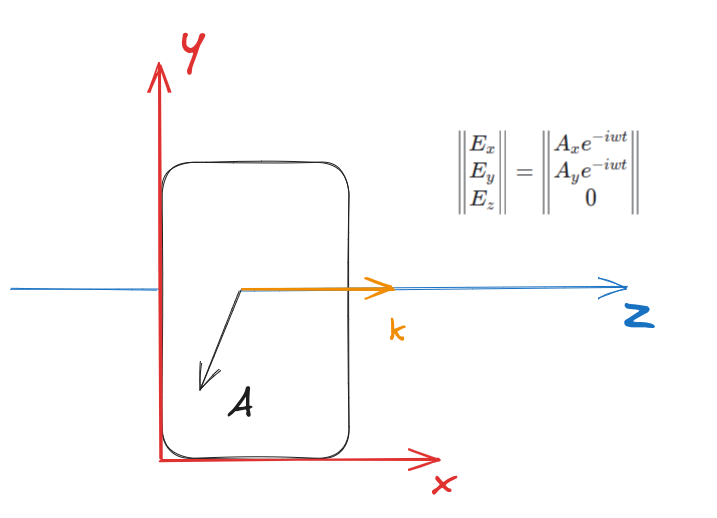
\includegraphics[width=0.6\textwidth]{stokes_1.png}
  \caption{Распространение электромагнитной волны. Вектор $\vec{E}$ перпендикулярен волновому вектору}
  \label{fig:wave}
\end{figure}

Из курса электричества мы знаем, что распространение электромагнитной волны описывается следующим выражением:
$$
\nabla^{2} E(x, t) - \frac{1}{c^{2}} \frac{\partial E}{\partial t^{2}} = 0
\label{wave_equation}
$$

Решением данного дифференциального уравнения является вектор:
$$
\begin{Vmatrix}   
E_{x} \\
E_{y} \\
E_{z}

\end{Vmatrix}= 
\begin{Vmatrix}   
A_{x} e^{i[(\vec{k}, \vec{r}) - wt]} \\
A_{y} e^{i[(\vec{k}, \vec{r}) - wt]}\\
A_{z} e^{i[(\vec{k}, \vec{r}) - wt]}

\end{Vmatrix}
$$

Подставив этот результат в уравнения Максвелла понимаем, что вектор амплитуды и вектор распространения волны перпендикулярны друг - другу: $(\vec{k}, \vec{A}) = 0$

Но тогда, поляризация вектора может быть задана при помощи лишь двух чисел $A_{x}, A_{y}$(см рисунок \ref{fig:wave}). Таким образом, числа $A_{x}$ и $A_{y}$ могут полностью задать поляризацию электромагнитной волны. Обычно их записывают в виде вектора, который называется \textbf{вектором Джонса}.




\begin{tcolorbox}[enhanced,attach boxed title to top center={yshift=-3mm,yshifttext=-1mm},colback=cyan!5!white,colframe=cyan!75!black,colbacktitle=cyan!80!black,title = Определение ,fonttitle=\bfseries, boxed title style={size=small,colframe=cyan!75!black} ]
    \textbf{\textcolor{href}{Вектор Джонса}} - вектор, направление которого соответствует направлению колебаний электрического поля света в плоскости, перпендикулярной направлению распространения света
\end{tcolorbox}

Круговая и эллиптическая поляризации тоже могут быть описаны при помощи математического формализма Джонса. При круговой поляризации амплитуды напряженности электрического поля по осям $x$ и $y$ равны, а их колебания происходят со сдвигом на $\pi / 2$. Набег фазы можем представить при помощи умножения на мнимую единицу:
$$
Re\{ie^{-iwt}\} = Re\{i(cos(-wt) + isin(-wt))\} = Re\{icos(wt) + sin(wt)\} = sin(wt)
$$

Так, вектор Джонса $J = [1, i]^{T}$ описывает круговую поляризацию, при которой вектор $\vec{E}$ вращается по часовой стрелке. Выражения векторов Джонса для различных эллиптических поляризаций выводятся из похожих соображений. Примеры приведены на рисунке \ref{fig:jones_polarizations}. 

\begin{figure}[htbp]
  \centering
  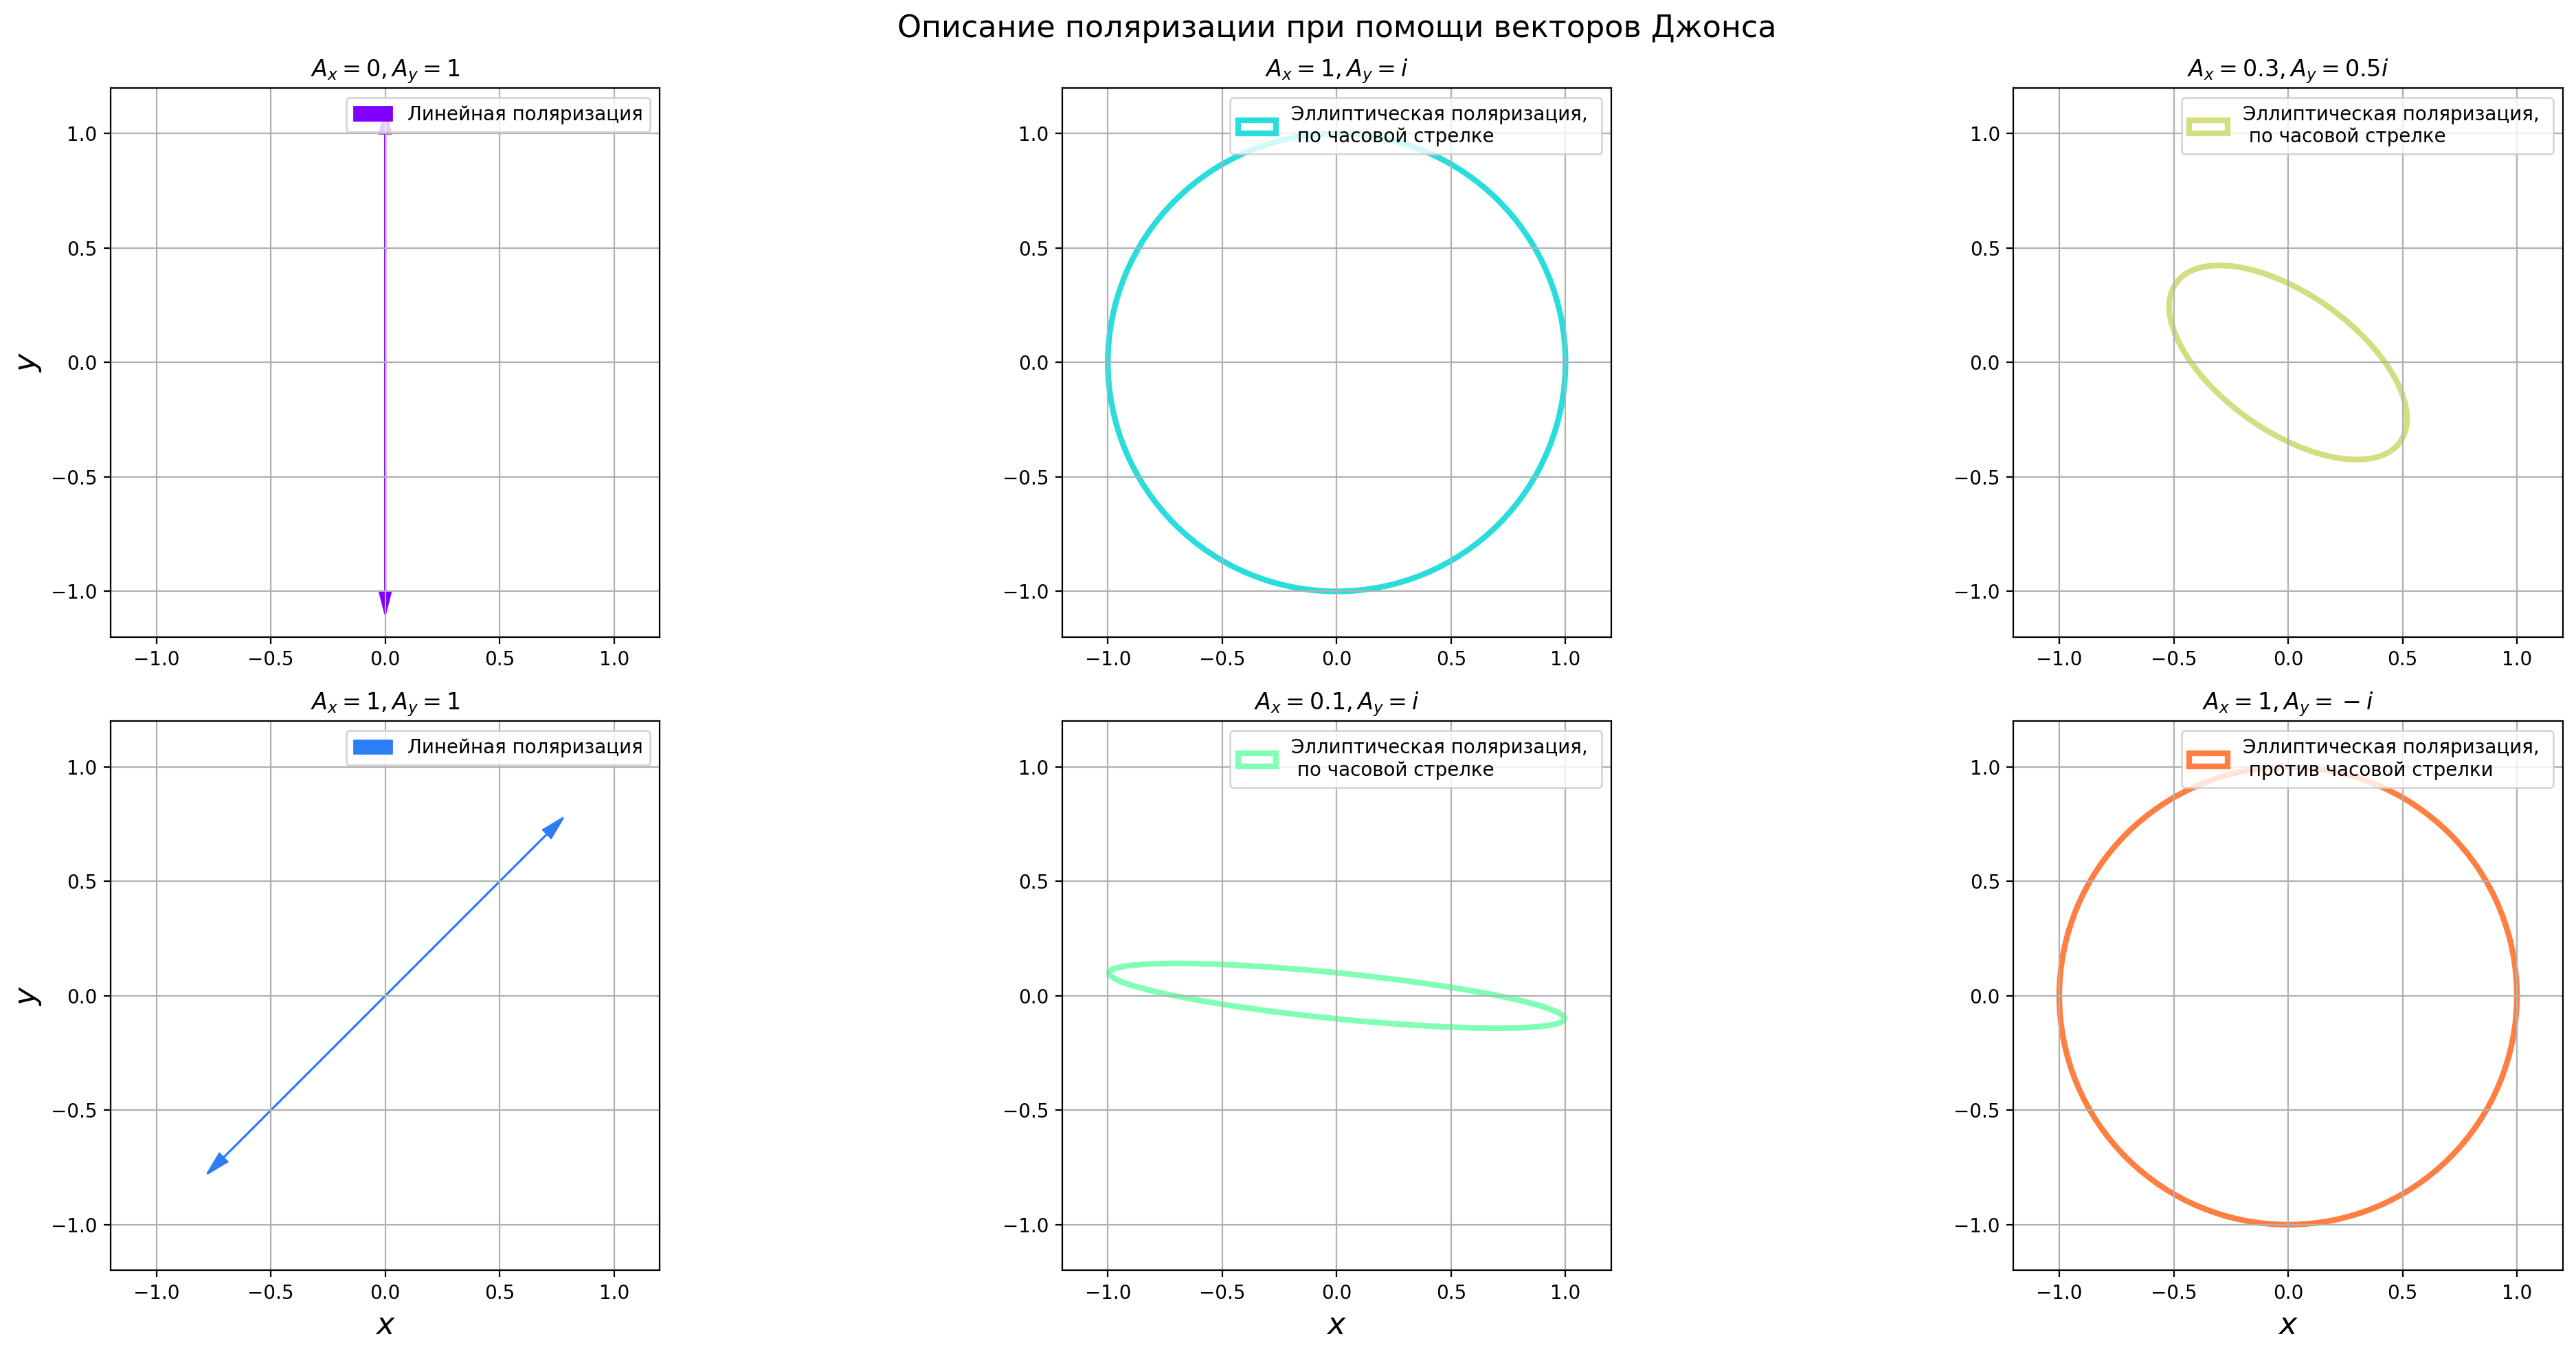
\includegraphics[width= 1\textwidth]{jones.png}
  \caption{Описание поляризации при помощи векторов Джонса}
  \label{fig:jones_polarizations}
\end{figure}



Джонсом также был придуман и математический аппарат для описания действия оптических элементов.

Пусть линейно поляризованный свет $J = [A_x, A_y]^{T}$($A_{x}, A_{y} \in R$) падает на поляроид, ось которого коллинеарна оси $y$. Свет вышедший из поляроида описывается вектором $J = [0, A_y]^{T}$. Действие поляроида на свет можно описать матрицей Джонса, представленной на рисунке \ref{fig:polaroid_responce_matrix}.

\newpage

\begin{figure}[htbp]
  \centering
  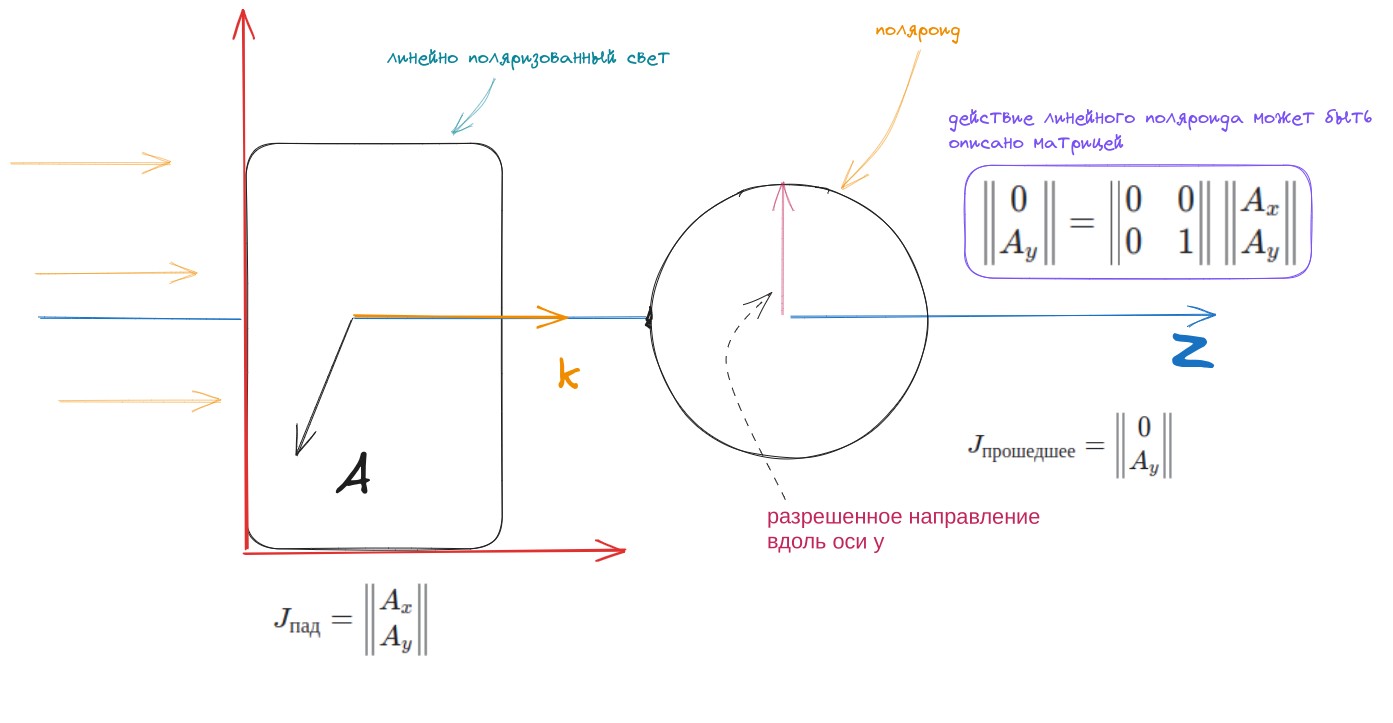
\includegraphics[width= 0.6\textwidth]{stokes_2.png}
  \caption{Использование матрицы Джонса для описания действия поляроида}
  \label{fig:polaroid_responce_matrix}
\end{figure}

Матрицы Джонса, описывающие действие других оптических элементов приведены на рисунке \ref{fig:jones_matricies_examples}. Прелесть матриц Джонса заключается в том, что к ним можно применять стандартные линейные операторы. Например, повёрнутый на $\theta$ поляроид описывается матрицей Джонса на которую подействовали оператором поворота: $W_{\theta} M W_{\theta}^{-1} = W_{\theta} M W_{-\theta}$(здесь $W \in 2 \times 2 $ - матрица поворота, $M$ - исходная матрица Джонса). 

\begin{figure}[htbp]
  \centering
  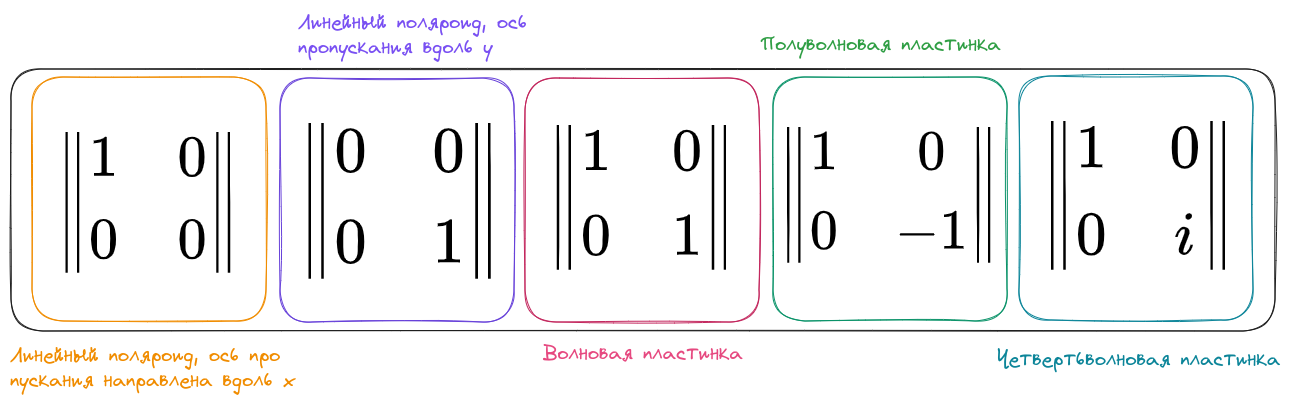
\includegraphics[width= 0.6\textwidth]{polaroid_table.png}
  \caption{Матрицы Джонса, описывающие действие линейных оптических элементов}
  \label{fig:jones_matricies_examples}
\end{figure}

\hspace*{1em}
\chapter*{Методика}

\subsection*{\textcolor{pink}{Оборудование}}
\begin{itemize}
    \item Поляроиды
    \item Кристалл...
    \item Сервопривод
    \begin{description}
     \item[Замечание:] Лучше использовать сервопривод постоянного вращения с установленной обратной связью
     \end{description}
    \item Микроконтроллер(atmega328pb)
    \item Программное обеспчение
    \begin{itemize}
        \item arduino ide
        \item Интерпретатор python
        \item Библиотека numpy - для вычислений и матричных операций
        \item openCV - автоматизация эксперимента, обработка изображений
        \item pySerial - автоматизация эксперимента
        \item matplotlib - построение графиков, визуализация данных
        \item scipy - аппроксимация полученных данных
    \end{itemize}
\end{itemize}

\subsection*{\textcolor{pink}{Эксперимент 1 - крутящаяся фигня с поляроидами}}
\subsection*{\textcolor{pink}{Эксперимент 2 - кристалл}}

\begin{tcolorbox}[enhanced,attach boxed title to top center={yshift=-3mm,yshifttext=-1mm},colback=cyan!5!white,colframe=cyan!75!black,colbacktitle=cyan!80!black,title =  Можем использовать вот такую красивую рамочку,fonttitle=\bfseries, boxed title style={size=small,colframe=cyan!75!black} ]
    Текст в рамочке
\end{tcolorbox}


\begin{tcolorbox}[enhanced,frame style image=blueshade.png,
  opacityback=0.75,opacitybacktitle=0.25,
  colback=blue!5!white,colframe=blue!75!black,
  title={\bf \centering И вот такую не очень красивую(как по мне) рамочку}]
    Текст в некрасивой рамочке
\end{tcolorbox}

% template to insert figure
%
%\begin{figure}[htbp]
%  \centering
%  \includegraphics[width=0.6\textwidth]
%{figurefilenamehere}
%  \caption{caption}
%\end{figure}


\end{document}
